\documentclass[11pt,a4paper]{article}
\usepackage[spanish,es-noshorthands]{babel}
\usepackage[utf8]{inputenc}
\usepackage[T1]{fontenc}
\usepackage[margin=2.2cm]{geometry}
\usepackage{amsmath,booktabs,graphicx,float,xcolor,listings,tikz,hyperref,caption}
\usetikzlibrary{positioning,arrows.meta,fit}
\setlength{\parindent}{0pt}
\setlength{\parskip}{5pt}
\captionsetup{font=small,labelfont=bf}
\hypersetup{colorlinks,linkcolor=black,urlcolor=blue!50!black,citecolor=black}

% Marca visible para lo que falta completar con resultados reales
\newcommand{\pendiente}[1]{\textbf{\color{red!70!black}[Pendiente: #1]}}
% Inserta una figura solo si ya existe (las figuras se generan con sim_todo.sh)
\newcommand{\figura}[3]{%
  \IfFileExists{#1}{\begin{figure}[H]\centering\includegraphics[width=#2\linewidth]{#1}\caption{#3}\end{figure}}%
  {\pendiente{figura \detokenize{#1}}}}

\lstset{basicstyle=\ttfamily\footnotesize,frame=single,breaklines=true,columns=fullflexible,
        keywordstyle=\bfseries,commentstyle=\color{gray},showstringspaces=false,
        literate={á}{{\'a}}1 {é}{{\'e}}1 {í}{{\'i}}1 {ó}{{\'o}}1 {ú}{{\'u}}1 {ñ}{{\~n}}1 {Á}{{\'A}}1 {É}{{\'E}}1 {Ó}{{\'O}}1 {Ñ}{{\~N}}1}

\title{\textbf{Laboratorio 6: LED con PS y PL, simulación de FFT y filtro FIR\\y consumo de potencia en la Arty Z7-20}}
% Autores: informe_grupal.tex redefine este comando antes de cargar este archivo
\providecommand{\autores}{Alumno: Ricardo Amiel Acuña Villogas}
\author{\autores}
\date{\today}

\begin{document}
\maketitle

\begin{abstract}
Se implementó en la Arty Z7-20 un sistema que enciende LEDs desde la lógica programable (PL) y desde el procesador ARM (PS), se simularon los núcleos xFFT y FIR Compiler de AMD y se estimó el consumo de potencia de los tres diseños con Vivado 2025.2. El diseño del LED funcionó en la placa: dos LEDs responden al programa en C y dos a la lógica de la FPGA, con un uso menor al 1 \% de los recursos. La FFT de 1024 puntos ubicó el tono de 1 MHz en el índice 10 y la transformada inversa reconstruyó la entrada con una similitud de 0.99999. La potencia total estimada fue de 1.401 W para el LED, 1.532 W para la FFT y 1.498 W para el FIR; en los tres casos el PS7 consume cerca de 1.26 W, por lo que el costo propio de la lógica de procesamiento es de solo 7, 127 y 92 mW respectivamente.
\end{abstract}

\section*{Material complementario}
\begin{itemize}
  \item Repositorio con el código, los scripts y este informe: \url{https://github.com/ricardoamiel/Arty-ZYNQ-7000---Laboratorio-6}
  \item Video de la placa en funcionamiento: \href{https://drive.google.com/file/d/15j47dAb3DASq5ieea0aM342emI3dTVuM/view?usp=sharing}{ver video en Drive}
  \item Carpeta con todo el material del laboratorio: \href{https://drive.google.com/drive/folders/1psmLtL21YHwi7eiOAoLBj23YtwVGnrsq?usp=sharing}{carpeta en Drive}
\end{itemize}

\section{Introducción}
La Arty Z7-20 usa el SoC Zynq-7000 XC7Z020, que integra en un mismo chip un sistema de procesamiento (PS) con dos núcleos ARM Cortex A9 y una lógica programable (PL) equivalente a una FPGA Artix 7. El PS ejecuta software en C y la PL implementa hardware dedicado; ambos se comunican por los buses AXI. Esta división permite repartir una tarea de procesamiento de señales: la PL ejecuta en paralelo las operaciones costosas, como la FFT o un filtro FIR, y el PS controla, configura y almacena los resultados.

El arranque del Zynq sigue dos etapas. Primero la BootROM carga el FSBL, que configura el PS y programa el bitstream en la PL. Luego se ejecuta la aplicación, ya sea un programa standalone en C o un sistema Linux mediante U Boot. En este laboratorio se usa la ruta standalone, programada por JTAG, que es suficiente para controlar periféricos y probar núcleos de procesamiento sin un sistema operativo.

\section{Objetivos}
\begin{enumerate}
  \item Diseñar un sistema que encienda LEDs desde la FPGA (PL) y desde el procesador (PS) de la Arty Z7-20.
  \item Simular los núcleos de propiedad intelectual xFFT y FIR Compiler de AMD y verificar su respuesta.
  \item Modificar la inyección de datos del ARM hacia la FPGA, de una señal senoidal a una señal cuadrada, y verificar la FFT y la IFFT calculadas por el núcleo.
  \item Documentar los diagramas de bloques de Vivado y los diagramas de tiempo de las interfaces AXI4 Stream.
  \item Estimar y analizar el consumo de potencia de los diseños implementados.
\end{enumerate}

\section{Materiales y herramientas}
\begin{itemize}
  \item Placa Digilent Arty Z7-20 (XC7Z020CLG400-1), cable micro USB y jumper JP4 en modo JTAG.
  \item Vivado ML Standard 2025.2 y Vitis Embedded Development 2025.2 en Ubuntu 24.04, con instalación mínima: solo la familia Zynq-7000 (descarga de 23 GB frente a los 163 GB de una instalación completa).
  \item Archivos de placa de Digilent (vivado-boards) para la Arty Z7-20.
  \item Python 3.12 con NumPy y Matplotlib para el posprocesamiento de la simulación.
\end{itemize}

\subsection{Migración del proyecto del curso a Linux y Vivado 2025.2}
Los scripts entregados por el docente fueron hechos para Windows y Vivado 2024.2. Para ejecutarlos en Ubuntu con la versión 2025.2 se hicieron los cambios de la Tabla \ref{tab:migracion}; ninguno altera la configuración de los núcleos ni del diseño de bloques.
\begin{table}[H]\centering
\caption{Adaptaciones hechas a los scripts del curso.}
\label{tab:migracion}
\begin{tabular}{p{0.38\linewidth}p{0.55\linewidth}}\toprule
Problema & Solución\\\midrule
Los scripts de bloques se detienen si la versión no es 2024.2 & La versión esperada se toma de la herramienta instalada; las versiones de los núcleos (xFFT 9.1, FIR 7.2, AXI DMA 7.1) no cambian en 2025.2\\
Rutas de Windows y llamadas a vivado.bat & entorno.sh ubica Vivado, Vitis y Python en cualquier instalación de Linux\\
Rutas con espacios cortadas por add\_files y get\_files & Las rutas se pasan como lista de Tcl\\
Board files instaladas dentro de Vivado & Se cargan desde la carpeta boards del proyecto con board.repoPaths\\
Simulación con interfaz gráfica obligatoria & Versión por lotes dsp\_sim\_batch.tcl y figuras vectoriales en Python\\
Memoria insuficiente al sintetizar con todos los núcleos & Se limitan los trabajos paralelos a 3 (variable VIVADO\_JOBS)\\\bottomrule
\end{tabular}
\end{table}

\section{Parte 1: encendido de LEDs con la FPGA y el procesador}
\subsection{Arquitectura}
El diseño de bloques contiene el PS7 configurado con el preajuste de la placa, un AXI GPIO de 2 bits conectado al puerto maestro M\_AXI\_GP0 y un módulo RTL propio. La Figura \ref{fig:arq_led} resume las conexiones.

\begin{figure}[H]\centering
\begin{tikzpicture}[font=\small, node distance=8mm and 12mm,
  b/.style={draw, rounded corners, minimum height=10mm, minimum width=26mm, align=center},
  a/.style={-{Latex[length=2mm]}, thick}]
  \node[b, fill=blue!8] (ps) {PS7\\ARM Cortex A9\\led\_main.c};
  \node[b, right=of ps] (ic) {AXI\\Interconnect};
  \node[b, right=of ic, fill=green!8] (gpio) {AXI GPIO\\2 bits};
  \node[b, below=of ic, fill=orange!10] (blink) {pl\_blink.v\\contador 1 Hz};
  \node[right=of gpio, align=left] (l01) {LD0 (R14)\\LD1 (P14)};
  \node[right=of blink, align=left] (l23) {LD2 (N16)\\LD3 (M14)};
  \node[below=6mm of blink] (sw) {SW0 (M20)};
  \draw[a] (ps) -- node[above]{GP0} (ic);
  \draw[a] (ic) -- (gpio);
  \draw[a] (gpio) -- (l01);
  \draw[a] (ps.south) |- node[pos=0.25,left]{FCLK0 100 MHz} (blink.west);
  \draw[a] (sw) -- (blink);
  \draw[a] (blink) -- (l23);
  \node[draw, dashed, fit=(gpio)(blink)(ic), inner sep=4mm, label={[anchor=north east]north east:PL}] {};
\end{tikzpicture}
\caption{Arquitectura del diseño: LD0 y LD1 los controla el procesador; LD2 y LD3 los controla solo la lógica programable.}
\label{fig:arq_led}
\end{figure}

\begin{figure}[H]\centering
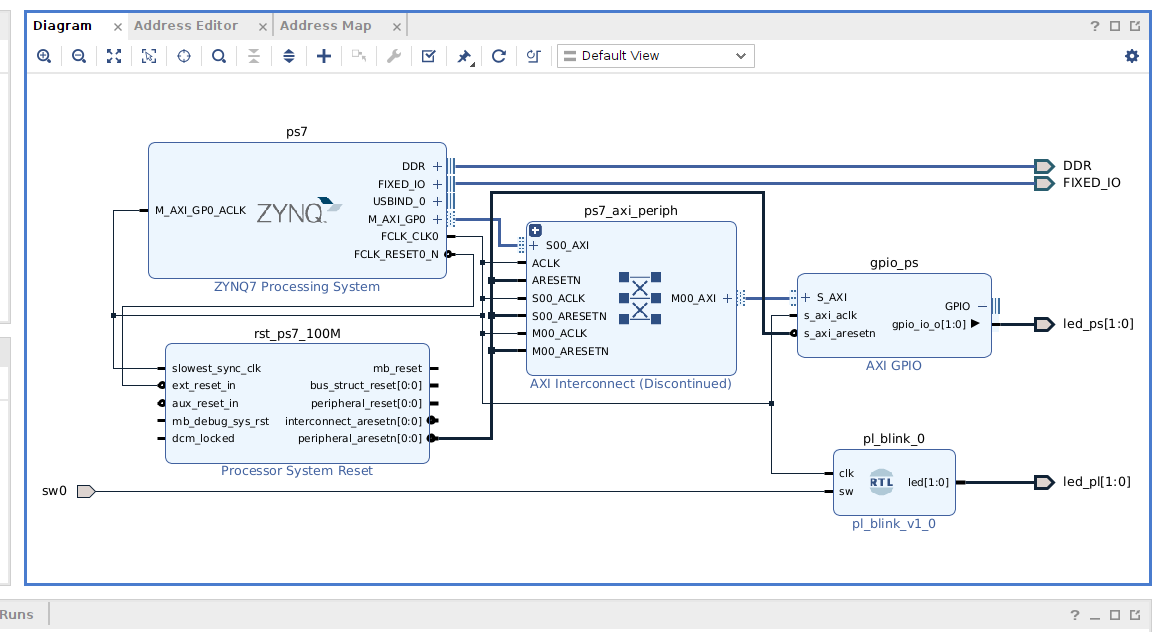
\includegraphics[width=0.95\linewidth]{figuras/block_design.png}
\caption{Diseño de bloques generado en Vivado 2025.2: PS7, AXI Interconnect, AXI GPIO (gpio\_ps), reinicio del procesador (rst\_ps7\_100M) y el módulo RTL pl\_blink\_0.}
\label{fig:bd}
\end{figure}

\subsection{Lógica programable (PL)}
El módulo pl\_blink divide el reloj FCLK0 de 100 MHz con un contador de 32 bits; cada 50 millones de ciclos invierte la salida, de modo que LD2 parpadea a 1 Hz sin intervención del procesador. LD3 copia directamente el estado del switch SW0.

\lstinputlisting[language=Verilog,caption={Módulo pl\_blink.v}]{../LED/hdl/pl_blink.v}

\subsection{Sistema de procesamiento (PS)}
El programa standalone inicializa el AXI GPIO y escribe cada 500 ms un patrón de dos bits: LD0 cambia en cada iteración y LD1 cada dos, lo que forma un contador binario visible. Cada iteración se reporta por la UART a 115200 baudios.

\lstinputlisting[language=C,caption={Programa led\_main.c}]{../LED/src/led_main.c}

\subsection{Flujo de implementación}
\begin{enumerate}
  \item Vivado crea el diseño de bloques, sintetiza, implementa y genera el bitstream y el archivo de plataforma sys\_wrapper.xsa (script led\_hw.tcl).
  \item Vitis crea la plataforma standalone a partir del .xsa y compila la aplicación (create\_vitis\_led.py).
  \item XSDB programa el bitstream, inicializa el PS con ps7\_init y descarga el ejecutable al Cortex A9 (program.tcl).
\end{enumerate}

Los tres pasos se ejecutaron por terminal con run\_led.sh (hw, sw y prog). Las Figuras \ref{fig:vivado}, \ref{fig:vitis} y \ref{fig:prog} muestran el resultado en cada herramienta.

\begin{figure}[H]\centering
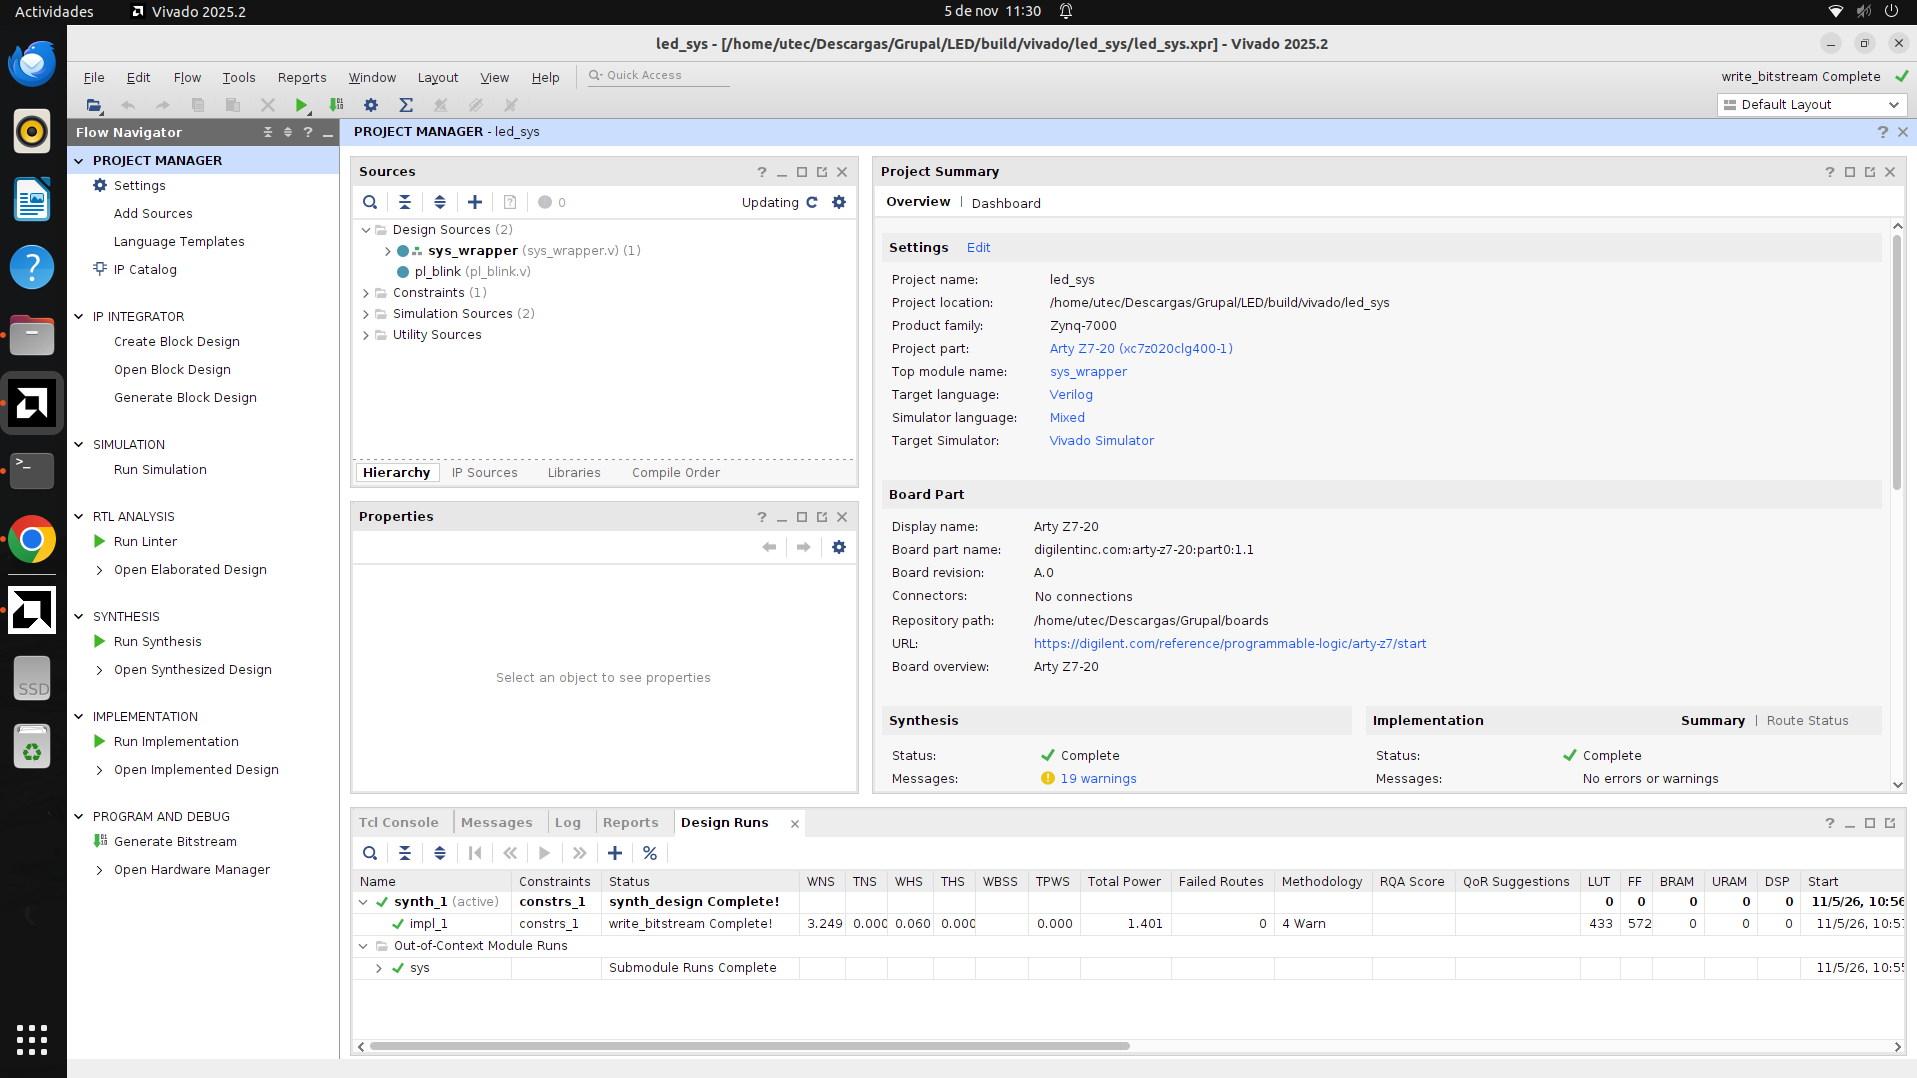
\includegraphics[width=0.95\linewidth]{figuras/vivado_resumen.png}
\caption{Resumen del proyecto en Vivado: placa Arty Z7-20, síntesis e implementación completas y bitstream generado.}
\label{fig:vivado}
\end{figure}

\begin{figure}[H]\centering
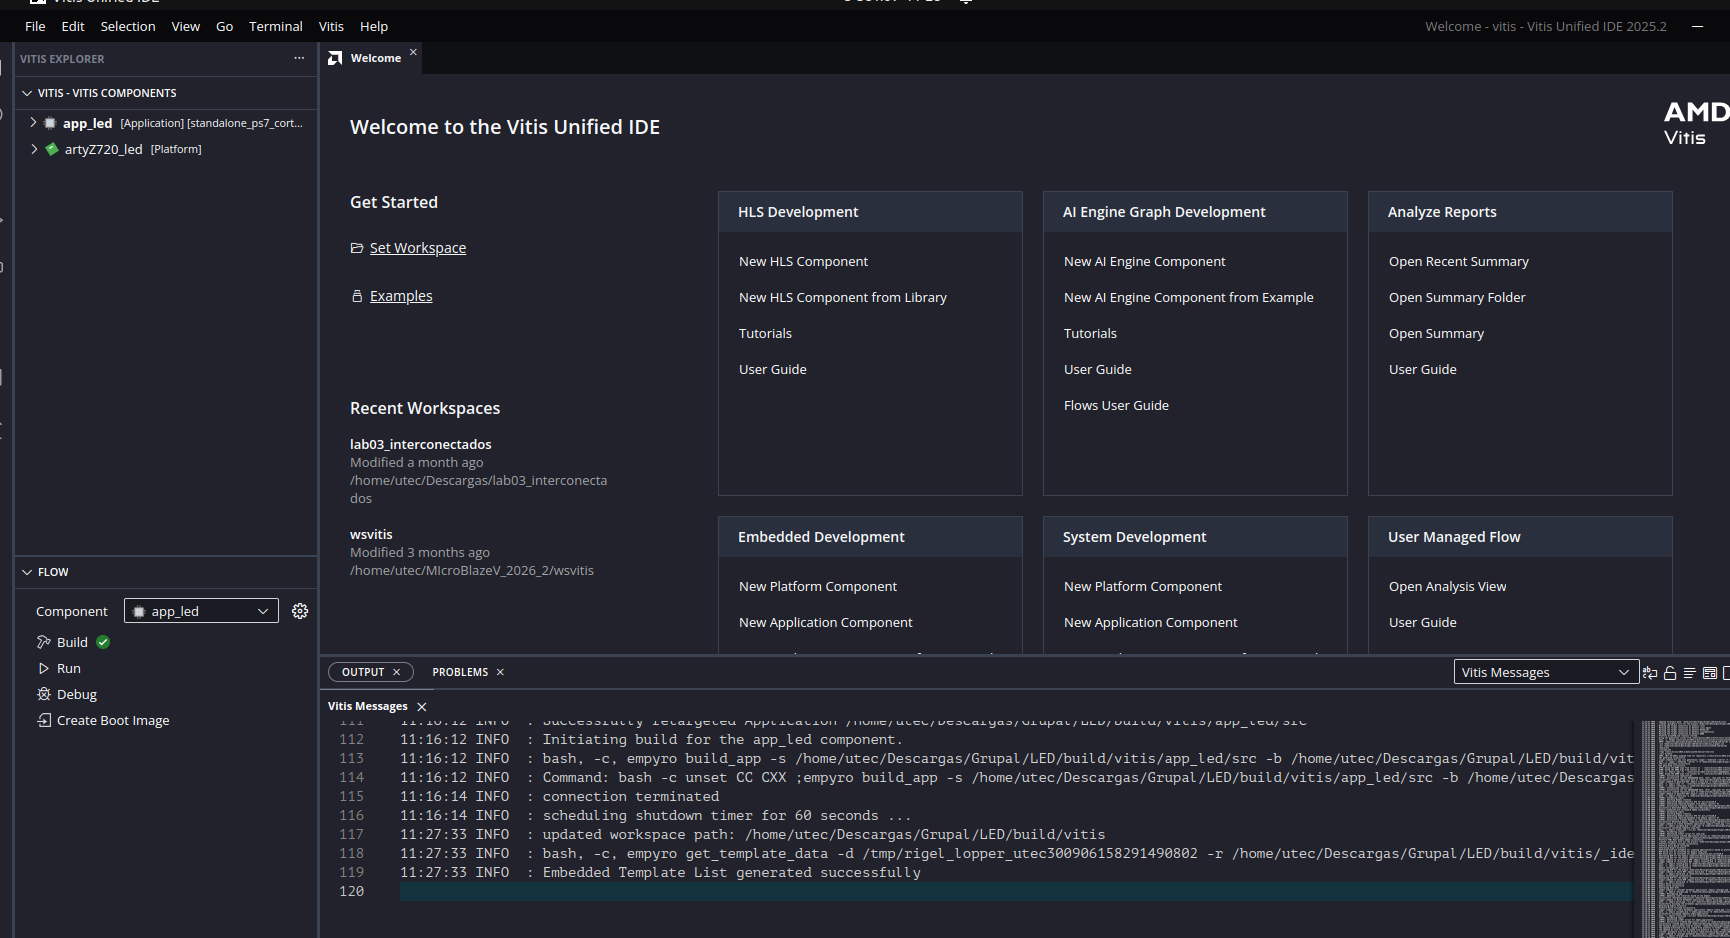
\includegraphics[width=0.95\linewidth]{figuras/vitis_ide.png}
\caption{Vitis Unified IDE 2025.2 con la plataforma artyZ720\_led y la aplicación app\_led compiladas.}
\label{fig:vitis}
\end{figure}

\begin{figure}[H]\centering
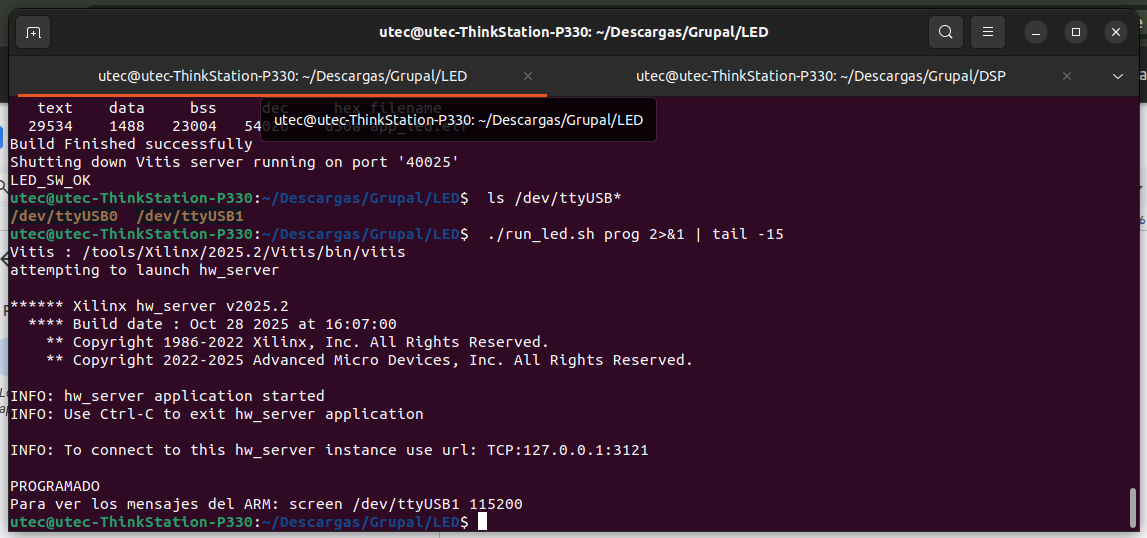
\includegraphics[width=0.8\linewidth]{figuras/terminal_prog.png}
\caption{Compilación de la aplicación y programación de la placa por JTAG con xsdb y hw\_server 2025.2.}
\label{fig:prog}
\end{figure}

\subsection{Resultados}
\begin{figure}[H]\centering
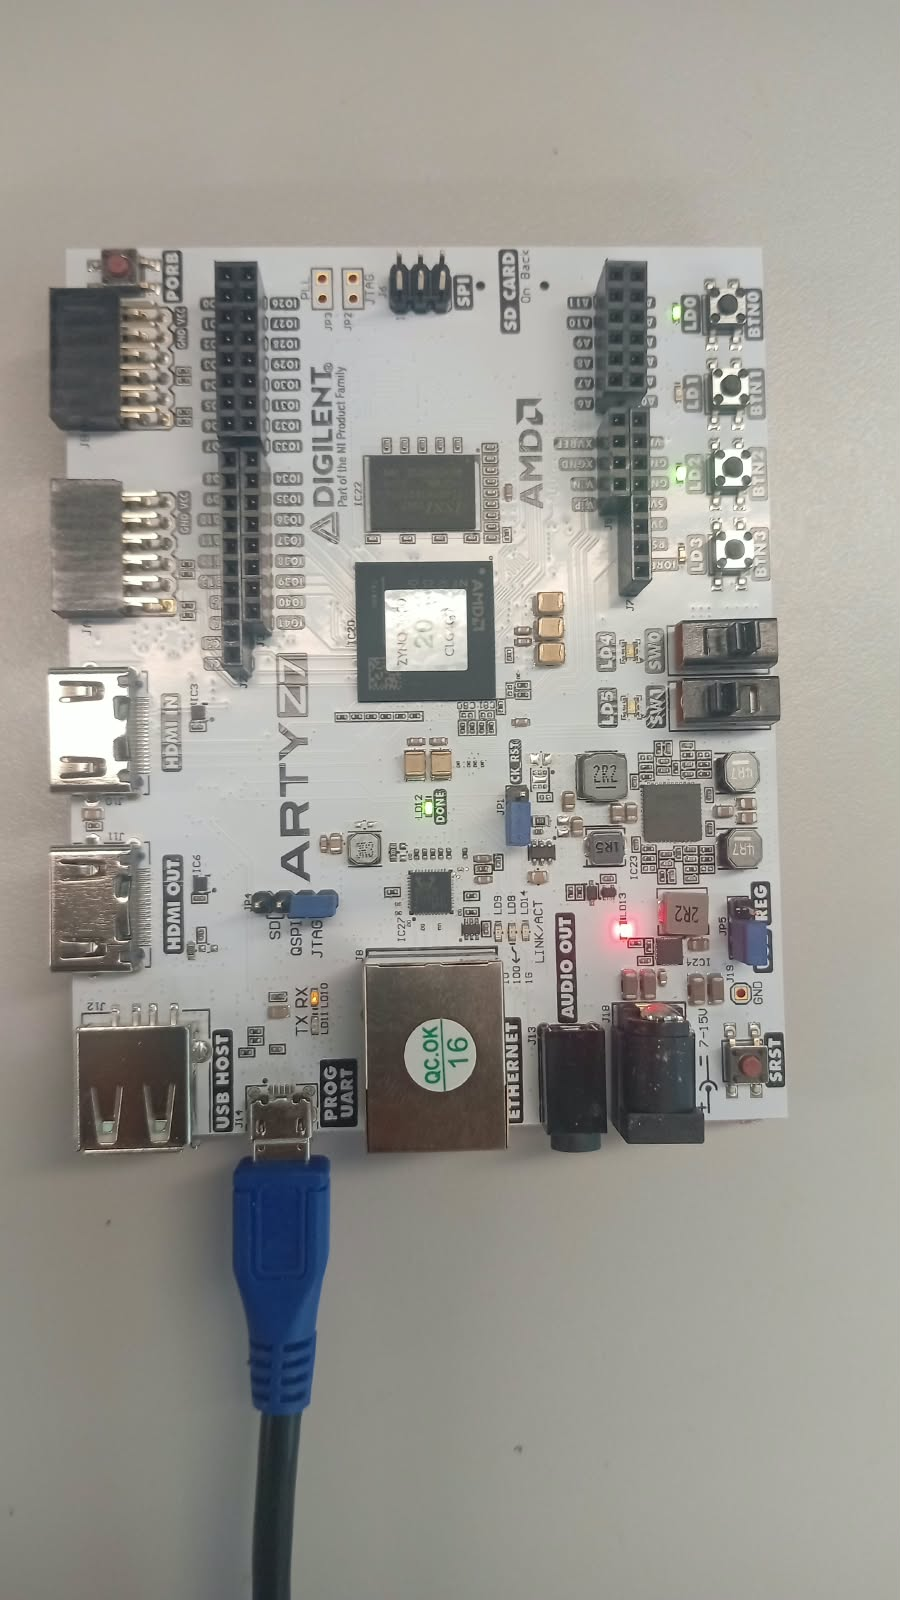
\includegraphics[width=0.5\linewidth]{figuras/arty_funcionando.jpeg}
\caption{Arty Z7-20 ejecutando el diseño. LD0 encendido por el procesador, LD2 encendido por el contador de la PL, LD3 apagado con SW0 abajo, LD12 (DONE) indica la FPGA configurada y el LED TX muestra la transmisión por la UART.}
\label{fig:arty}
\end{figure}

La consola serial (115200 baudios) muestra la secuencia que escribe el procesador, que coincide con lo observado en LD1 y LD0 (Figura \ref{fig:uart}).

\begin{figure}[H]\centering
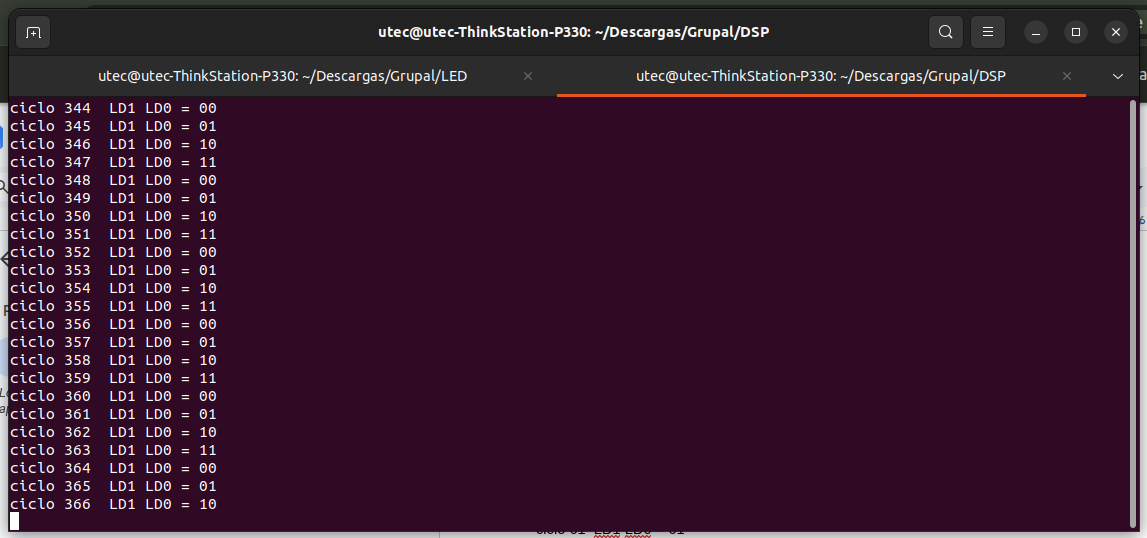
\includegraphics[width=0.75\linewidth]{figuras/consola_uart.png}
\caption{Salida de la UART: el procesador recorre el contador de dos bits 00, 01, 10, 11 cada 500 ms.}
\label{fig:uart}
\end{figure}

El video de la placa en funcionamiento (ver enlaces en Material complementario) muestra el parpadeo de LD2 a 1 Hz independiente del contador del procesador y la respuesta de LD3 al switch SW0.

\begin{table}[H]\centering
\caption{Recursos y tiempos del diseño del LED (Vivado, implementación).}
\label{tab:recursos_led}
\begin{tabular}{lcc}\toprule
Recurso & Usado & Disponible en XC7Z020\\\midrule
LUT & 433 & 53200\\
Flip flops & 572 & 106400\\
BRAM & 0 & 140\\
DSP & 0 & 220\\\midrule
WNS (holgura de setup) & \multicolumn{2}{c}{3.249 ns}\\
WHS (holgura de hold) & \multicolumn{2}{c}{0.060 ns}\\\bottomrule
\end{tabular}
\end{table}
El diseño usa menos del 1 \% de la lógica disponible y cumple las restricciones de tiempo a 100 MHz, ya que ambas holguras son positivas. La mayor parte de las LUT y flip flops corresponden al AXI Interconnect y al AXI GPIO; el contador de pl\_blink solo requiere 33 registros.

\section{Parte 2: simulación de la FFT y del filtro FIR}
\subsection{Configuración de los núcleos}
\begin{table}[H]\centering
\caption{Parámetros principales de los núcleos simulados (dsp\_sim.tcl).}
\begin{tabular}{lll}\toprule
Núcleo & Parámetro & Valor\\\midrule
xFFT 9.1 & Longitud máxima / usada & 2048 / 1024 puntos (configurable en ejecución)\\
 & Arquitectura & Pipelined streaming I/O\\
 & Datos de entrada / factores de fase & 16 bits / 24 bits\\
 & Orden de salida & Natural\\
 & Reloj & 100 MHz\\\midrule
FIR Compiler 7.2 & Pasabanda & Coeficientes BPF.coe, 16 bits\\
 & Hilbert & Coeficientes hilbert\_0.coe\\
 & Decimador & Factor 4, LPF\_dec.coe\\
 & Interpolador & Factor 4, LPF\_int.coe\\
 & Arquitectura & Systolic multiply accumulate\\\bottomrule
\end{tabular}
\end{table}

\subsection{Estímulos}
Para la FFT el testbench genera un tono complejo de 1 MHz muestreado a 100 MHz en un bloque de 1024 muestras; el resultado de la transformada directa entra a una segunda instancia configurada como transformada inversa. Para el FIR se inyectan 1024 muestras de ruido aleatorio, cuyo espectro plano permite observar la respuesta en frecuencia de cada filtro.

Con $f_s = 100$ MHz y $N = 1024$, la resolución en frecuencia es
\[
\Delta f = \frac{f_s}{N} = \frac{100\ \text{MHz}}{1024} \approx 97.66\ \text{kHz},
\]
por lo que el tono de 1 MHz debe aparecer cerca del índice $k = 1\ \text{MHz}/\Delta f \approx 10.24$.

\subsection{Resultados de la FFT}
\figura{../DSP/resultados/xfft_1.pdf}{0.95}{Entrada, salida de la FFT directa y salida de la FFT inversa del núcleo xFFT.}
La salida directa concentra la energía en el índice $k = 10$, que corresponde a $10 \cdot 97.66 \approx 976.6$ kHz, el bin más cercano a 1 MHz. Como el tono cae en $k = 10.24$ y no en un entero, parte de la energía se reparte en los bins vecinos $k = 11$ y $k = 9$ (magnitudes de 2869 y 1755 frente a 9076 en el pico); esta es la fuga espectral propia de una ventana rectangular. El núcleo escala la salida por $1/1024$ para evitar desbordes en sus 16 bits: la relación entre el pico del hardware y el de numpy.fft es 0.00098, es decir, exactamente $1/N$.

La transformada inversa recupera la señal original: su amplitud máxima es 10054 frente a 10000 en la entrada y la similitud normalizada entre ambas señales es 0.99999. La pequeña diferencia proviene del redondeo en aritmética de punto fijo dentro de las dos transformadas.

\begin{table}[H]\centering
\caption{Verificación numérica de la FFT (datos de la simulación frente a numpy).}
\begin{tabular}{lc}\toprule
Magnitud & Valor\\\midrule
Índice del pico (hardware y numpy) & 10\\
Bins vecinos con fuga & 11 y 9\\
Escala del hardware respecto a numpy & 0.00098 $\approx 1/1024$\\
Similitud entrada frente a IFFT & 0.99999\\\bottomrule
\end{tabular}
\end{table}

\subsection{Resultados del filtro FIR}
\figura{../DSP/resultados/fir_compiler_1.pdf}{0.8}{Señal de entrada (ruido) al FIR Compiler.}
\figura{../DSP/resultados/fir_compiler_2.pdf}{0.8}{Salida del filtro pasabanda.}
\figura{../DSP/resultados/fir_compiler_3.pdf}{0.8}{Salida del interpolador.}
\figura{../DSP/resultados/fir_compiler_4.pdf}{0.8}{Salida del decimador.}
\figura{../DSP/resultados/fir_compiler_5.pdf}{0.8}{Salida del transformador de Hilbert (parte real e imaginaria).}
\figura{../capturas/bd_fir.pdf}{0.98}{Diagrama de bloques del sistema FIR exportado de Vivado 2025.2.}
\begin{itemize}
  \item Entrada: el ruido aleatorio tiene un espectro aproximadamente plano entre 0 y 50 MHz, por lo que sirve para observar la respuesta de cada filtro.
  \item Pasabanda: conserva la banda centrada en 10 MHz; el 90 \% de la energía de salida queda entre 6.9 y 13.1 MHz, y fuera de ella la atenuación es de unos 40 a 50 dB.
  \item Interpolador por 4: el filtro paso bajo elimina las imágenes espectrales que aparecen al insertar ceros; la salida conserva la banda baja hasta unos 10 MHz y atenúa el resto en más de 40 dB.
  \item Decimador por 4: filtra antes de submuestrear y la salida queda a 25 MHz con 256 muestras (1024 entre 4); su espectro ocupa de 0 a 12.5 MHz sin componentes plegadas visibles.
  \item Hilbert: entrega una parte real y una imaginaria desfasadas 90 grados para formar la señal analítica. Con ruido real a la entrada la supresión de frecuencias negativas medida es de solo 4.9 dB, porque el filtro solo actúa dentro de su banda de paso; con una señal de banda angosta el efecto sería más marcado.
\end{itemize}

\section{Parte 3: FFT en el sistema PS y PL con señal cuadrada}
\subsection{Diagrama de bloques del sistema FFT}
El diseño del curso conecta el procesador con el núcleo xFFT mediante un AXI DMA. El ARM escribe en la DDR la configuración y las muestras; el DMA las lee por el puerto HP0 y las entrega como flujo AXI4 Stream. Un AXI4 Stream Switch, controlado por el ARM, dirige ese flujo al canal de configuración del núcleo (a través de un convertidor de subconjunto que recorta la palabra a 24 bits) o al canal de datos. La salida de la FFT vuelve por el DMA a la DDR mediante el puerto HP1. Un System ILA observa la entrada y la salida del núcleo para depuración por JTAG.

\figura{../capturas/bd_xfft.pdf}{0.98}{Diagrama de bloques del sistema FFT exportado de Vivado 2025.2: PS7, AXI DMA, AXI4 Stream Switch, convertidor de subconjunto, xFFT 9.1 y System ILA.}
\figura{../capturas/bd_xfft.png}{0.98}{Captura de la interfaz de Vivado con el diagrama de bloques del sistema FFT.}

\subsection{Modificación de la inyección de datos: de senoidal a cuadrada}
La aplicación original del ARM generaba una señal compleja de barrido en frecuencia (chirp de 8 a 0 MHz) con amplitud 16000. Se reemplazó por una señal cuadrada real de la misma amplitud, con periodo de 64 muestras, es decir $f_0 = 100\ \text{MHz}/64 = 1.5625$ MHz. Con $N = 2048$ el periodo cabe un número entero de veces (32), por lo que la fundamental cae exactamente en el bin $k_0 = 32$ sin fuga espectral.

\lstinputlisting[language=C,caption={Función que genera la señal cuadrada en xfft\_main.c},linerange={318-331}]{../DSP/ip_xfft/xfft_main.c}

Además se corrigieron tres detalles del programa original que afectaban la lectura de resultados:
\begin{itemize}
  \item La salida de la IFFT se escribía sobre el buffer de entrada; ahora tiene su propio buffer en 0x10500000, de modo que entrada, FFT e IFFT quedan disponibles en la DDR.
  \item El puntero a la palabra de configuración nunca se inicializaba y apuntaba a la dirección 0; ahora apunta a una variable alineada.
  \item La espera del DMA terminaba cuando acababa cualquiera de los dos canales; ahora espera el canal que corresponde a cada etapa antes de leer el resultado.
\end{itemize}

\subsection{Verificación con los mismos datos del ARM}
Para verificar el cálculo de la FPGA se creó el testbench xfft\_square\_tb, que entrega al núcleo exactamente la misma secuencia que genera init\_tx\_buffer\_square, con la misma palabra de configuración: 2048 puntos, dirección directa y esquema de escalamiento 0x6AA para la FFT, y escalamiento nulo para la IFFT. El núcleo se simula con su modelo de comportamiento, que reproduce el cálculo en punto fijo del hardware.

\figura{../DSP/resultados/xfft_cuadrada_sim.pdf}{0.9}{Señal cuadrada inyectada, magnitud de la FFT calculada por el núcleo frente a numpy y reconstrucción con la IFFT.}

Una cuadrada de amplitud $A$ solo contiene armónicos impares, con amplitud proporcional a $1/m$:
\[
x(t) = \frac{4A}{\pi}\sum_{m=1,3,5,\dots}\frac{1}{m}\sin(2\pi m f_0 t)
\quad\Rightarrow\quad
|X[m k_0]| \approx \frac{2A}{\pi m}\ \text{(con la escala } 1/N\text{ del núcleo)}.
\]
\begin{table}[H]\centering
\caption{Magnitud de la FFT en los primeros armónicos (A = 16000).}
\label{tab:armonicos}
\begin{tabular}{cccccc}\toprule
$m$ & $k$ & $f$ (MHz) & Teoría $2A/(\pi m)$ & numpy escalado & Núcleo xFFT\\\midrule
1 & 32 & 1.5625 & 10186 & 10191.2 & 10191.2\\
2 & 64 & 3.1250 & 0 & 0 & 0\\
3 & 96 & 4.6875 & 3395 & 3408.0 & 3408.7\\
4 & 128 & 6.2500 & 0 & 0 & 0\\
5 & 160 & 7.8125 & 2037 & 2058.0 & 2058.4\\\bottomrule
\end{tabular}
\end{table}
El núcleo coincide con numpy con un error máximo relativo de 0.02 \%, producto del redondeo en punto fijo. El esquema 0x6AA escala la salida por $1/2048 = 1/N$, lo que evita el desborde de los 16 bits. Las pequeñas diferencias frente a la teoría continua se deben al solapamiento de los armónicos superiores en una señal muestreada. La IFFT sin escalamiento devuelve la cuadrada original con amplitud máxima de 16006 y similitud normalizada de 1.000000.

\subsection{Diagramas de tiempo}
Los diagramas se obtuvieron del volcado VCD de la simulación. Todas las interfaces usan AXI4 Stream a 100 MHz: una muestra se transfiere en cada flanco de subida de aclk en que tvalid y tready valen 1 a la vez.

\figura{../DSP/resultados/diagrama_tiempo_general.pdf}{0.98}{Diagrama de tiempo completo: configuración del núcleo, trama de entrada de 2048 muestras, salida de la FFT y salida de la IFFT.}
\figura{../DSP/resultados/diagrama_tiempo_inicio.pdf}{0.98}{Inicio de la trama de entrada: el núcleo mantiene tready en 1 y acepta una muestra por ciclo; el bus de datos alterna entre 16000 y menos 16000 cada 32 muestras.}
\figura{../DSP/resultados/diagrama_tiempo_fin_trama.pdf}{0.98}{Fin de la trama de entrada: tlast se activa con la muestra 2048 y marca el fin de la trama.}
\figura{../capturas/ondas_xfft_sq.png}{0.98}{Captura del visor de ondas de Vivado con la simulación de la señal cuadrada.}

\begin{table}[H]\centering
\caption{Tiempos medidos en la simulación.}
\label{tab:tiempos}
\begin{tabular}{lc}\toprule
Evento & Tiempo\\\midrule
Primera muestra de entrada & 385 ns\\
Duración de la trama de entrada (2048 ciclos de 10 ns) & 20.48 µs\\
Primera muestra de salida de la FFT & 42.6 µs\\
Primera muestra de salida de la IFFT & 84.8 µs\\\bottomrule
\end{tabular}
\end{table}
La arquitectura pipelined streaming procesa una trama mientras recibe la siguiente, pero la salida en orden natural exige esperar a que llegue la trama completa y reordenar los resultados; por eso la FFT empieza a entregar datos unos 21.7 µs después de terminar la entrada, del orden de una trama adicional. La IFFT, conectada en cascada, repite el mismo retardo. Con ambos núcleos ocupados, el sistema puede sostener una muestra por ciclo, es decir 100 millones de muestras por segundo.

\subsection{Ejecución en la placa}
El bitstream del sistema FFT y la aplicación con la señal cuadrada quedaron compilados con Vivado y Vitis 2025.2. El script fft\_placa.sh graba la placa, ejecuta el programa en el ARM, lee de la DDR los tres buffers con xsdb y genera la misma figura con datos reales. \IfFileExists{../DSP/resultados/xfft_cuadrada_placa.pdf}{La Figura siguiente muestra el resultado obtenido en la Arty Z7-20.}{La ejecución en la placa queda pendiente porque la Arty Z7-20 no estuvo disponible al cierre de este informe; la verificación del cálculo se hizo con los mismos datos y la misma configuración mediante simulación.}
\figura{../DSP/resultados/xfft_cuadrada_placa.pdf}{0.9}{FFT e IFFT ejecutadas en la Arty Z7-20 con la señal cuadrada inyectada por el ARM.}

\section{Parte 4: consumo de potencia}
\subsection{Metodología}
La potencia se estimó con report\_power de Vivado sobre cada diseño implementado, con las condiciones por defecto (temperatura ambiente de 25 °C y actividad de conmutación vectorless de 12.5 \%). La potencia total se divide en estática, debida a las corrientes de fuga del chip, y dinámica, proporcional a la frecuencia y a la actividad:
\[
P_{din} = \alpha \, C \, V^2 f ,
\]
donde $\alpha$ es el factor de actividad, $C$ la capacitancia conmutada, $V$ la tensión de alimentación y $f$ la frecuencia de reloj.

\subsection{Resultados}
\begin{table}[H]\centering
\caption{Recursos usados por cada diseño implementado (XC7Z020).}
\label{tab:recursos}
\begin{tabular}{lccc}\toprule
Recurso & LED & FFT & FIR\\\midrule
LUT (de 53200) & 433 (0.8 \%) & 7660 (14.4 \%) & 6265 (11.8 \%)\\
Flip flops (de 106400) & 572 (0.5 \%) & 11736 (11.0 \%) & 11474 (10.8 \%)\\
BRAM (de 140) & 0 & 17 (12.1 \%) & 8.5 (6.1 \%)\\
DSP (de 220) & 0 & 20 (9.1 \%) & 57 (25.9 \%)\\\bottomrule
\end{tabular}
\end{table}
\begin{table}[H]\centering\caption{Resumen de potencia estimada por Vivado (report\_power).}\label{tab:pot_resumen}
\begin{tabular}{lccc}\toprule
Parámetro & LED (PS + PL) & FFT (xFFT + DMA) & FIR (4 filtros + DMA)\\\midrule
Potencia total en chip (W) & 1.401 & 1.532 & 1.498\\
Potencia dinámica (W) & 1.263 & 1.393 & 1.358\\
Potencia estática (W) & 0.137 & 0.139 & 0.141\\
Temperatura de unión (°C) & 41.2 & 42.7 & 42.3\\
\bottomrule\end{tabular}\end{table}
\begin{table}[H]\centering\caption{Potencia dinámica por componente (W).}\label{tab:pot_comp}
\begin{tabular}{lccc}\toprule
Componente & LED (PS + PL) & FFT (xFFT + DMA) & FIR (4 filtros + DMA)\\\midrule
Clocks & 0.003 & 0.042 & 0.038\\
Slice Logic & <0.001 & 0.021 & 0.006\\
Signals & 0.001 & 0.026 & 0.010\\
Block RAM & 0 & 0.021 & 0.003\\
DSPs & 0 & 0.018 & 0.034\\
I/O & 0.002 & 0 & <0.001\\
PS7 (procesador) & 1.256 & 1.266 & 1.266\\
\bottomrule\end{tabular}\end{table}
\begin{table}[H]\centering\caption{Potencia dinámica atribuible solo a la lógica programable (dinámica total menos PS7).}\label{tab:pot_pl}
\begin{tabular}{lccc}\toprule
 & LED (PS + PL) & FFT (xFFT + DMA) & FIR (4 filtros + DMA)\\\midrule
PL dinámica (W) & 0.007 & 0.127 & 0.092\\
\bottomrule\end{tabular}\end{table}


\subsection{Análisis}
\begin{enumerate}
  \item El PS7 domina el consumo. En los tres diseños el procesador aporta entre 1.256 y 1.266 W, más del 90 \% de la potencia total. Esa cifra incluye los dos núcleos Cortex A9, la memoria DDR3 y los periféricos fijos, y se mantiene casi igual porque la configuración del PS es la misma en todos los casos.
  \item La lógica del LED es casi gratuita. El contador y el AXI GPIO agregan solo 7 mW de potencia dinámica; la potencia estática de 0.137 W existe aunque la lógica no conmute.
  \item La FFT es el diseño de PL más costoso (127 mW). Necesita 17 bloques BRAM para guardar los datos y los factores de fase de 2048 puntos, y su reloj llega a muchos más registros; por eso Clocks, Signals y Block RAM superan a los del FIR.
  \item El FIR usa más DSP pero consume menos (92 mW). Sus cuatro filtros ocupan 57 DSP (26 \% del chip) en estructura sistólica, y los DSP son bloques de multiplicación dedicados más eficientes que la lógica general; además necesita la mitad de BRAM que la FFT.
  \item La temperatura de unión se mantiene entre 41 y 43 °C, muy por debajo del límite, con un margen de temperatura ambiente cercano a 68 °C.
  \item Los diseños de la FFT y del FIR incluyen el DMA y un System ILA para depuración por JTAG; el ILA usa BRAM y lógica que no serían necesarias en un diseño final, así que su consumo real sería algo menor.
\end{enumerate}

Para reducir el consumo se puede: bajar la frecuencia de FCLK0 o de los procesadores cuando la tarea lo permita, ya que la potencia dinámica es proporcional a $f$; deshabilitar los periféricos del PS que no se usan (USB, Ethernet, SD); retirar el ILA de la versión final; y reducir el ancho de los datos o la longitud máxima de la FFT a lo estrictamente necesario, lo que disminuye BRAM, DSP y capacitancia conmutada. Las cifras son estimaciones vectorless con actividad por defecto, con nivel de confianza alto en la implementación pero no medidas en la placa.

\section{Conclusiones}
\begin{enumerate}
  \item El Zynq permite controlar el mismo tipo de periférico desde dos dominios: los LEDs de la PL funcionan sin software y con tiempo exacto, mientras que los del PS se controlan con un programa en C a través del bus AXI; ambos convivieron en la placa sin interferencia.
  \item Los núcleos xFFT y FIR Compiler responden según lo esperado: la FFT ubica el tono en el bin correcto, muestra la fuga espectral prevista para un tono fuera de bin y la IFFT reconstruye la señal; cada filtro FIR moldea el espectro del ruido según su tipo.
  \item El consumo está dominado por el procesador (cerca de 1.26 W); la lógica de procesamiento añade entre 7 y 127 mW según el diseño, por lo que mover cálculos intensivos a la PL tiene un costo energético bajo frente al del PS.
  \item La instalación mínima de Vivado y Vitis 2025.2, limitada a la familia Zynq 7000, fue suficiente para todo el laboratorio y redujo la descarga de 163 GB a 23 GB.
\end{enumerate}

\begin{thebibliography}{9}
\bibitem{zynq} AMD, Zynq 7000 SoC Technical Reference Manual (UG585).
\bibitem{xfft} AMD, Fast Fourier Transform LogiCORE IP Product Guide (PG109).
\bibitem{fir} AMD, FIR Compiler LogiCORE IP Product Guide (PG149).
\bibitem{power} AMD, Vivado Design Suite User Guide: Power Analysis and Optimization (UG907).
\bibitem{arty} Digilent, Arty Z7 Reference Manual.
\end{thebibliography}

\end{document}
